%!/usr/bin/env pdflatex
%-*- coding: utf-8 -*-
%@author : Romain Graux
%@date : 2022 May 03, 12:22:56
%@last modified : 2022 June 17, 14:26:54

As we produce more data every year, it is becoming essential to store it as efficiently as possible. The current solution is to rely on electronic devices, organised in large data centers with an important energy consumption. For instance, the energy consumed by data centres in the European Union was of 76.8 TWh in 2018, which corresponds to 2.7\% of the total electricity demand for that year. Predictions estimate both the absolute number and relative share to increase to respectively 98,52 TWh and 3.21\% by 2030. As we can observe on Figure~\ref{fig:consumption}, it is not about to stop.

%https://digital-strategy.ec.europa.eu/en/library/energy-efficient-cloud-computing-technologies-and-policies-eco-friendly-cloud-market


%The U.S. department of Energy states that 2\% of the total U.S. electricity use.
%https://www.energy.gov/eere/buildings/data-centers-and-servers 

For both ecological and economical reasons, it is becoming increasingly interesting to find more efficient alternatives, such as DNA. Our genetic code packs billions of gigabytes into a single gram. A mere milligram of the molecule could encode the complete text of every book in the Library of Congress and have plenty of room to spare. \cite{bib:dna_data_storage}

Unfortunately, the present information retrieval latency and the high cost of the DNA sequencer among other instruments hinder a wide-spread application of DNA as storage. Currently, one cannot expect to replace a standard USB flash drive with a DNA-based variant without major changes to the experience. \cite{bib:dna_data_storage} Driven by the field's potential applications, promising developments are enabling cheaper, faster and smaller technology. 
% \illustrate{idéalement plusieurs refs avec les dernières avancées et leur application, les grands papiers du field}

% Since it is now possible to manipulate synthetic DNA \illustrate{Find an article talking about the first DNA synthesize}, it would be one of a new type 

Furthermore, the current disadvantages with DNA-based storage are not relevant for all applications. For instance, DNA based storage is convenient for long term media preservation archives (so called cold media storage) which are infrequently accessed and thus do not need low information retrieval latency. \cite{bib:Panda2018}

\subsection{DNA}

\begin{figure}
    \centering
    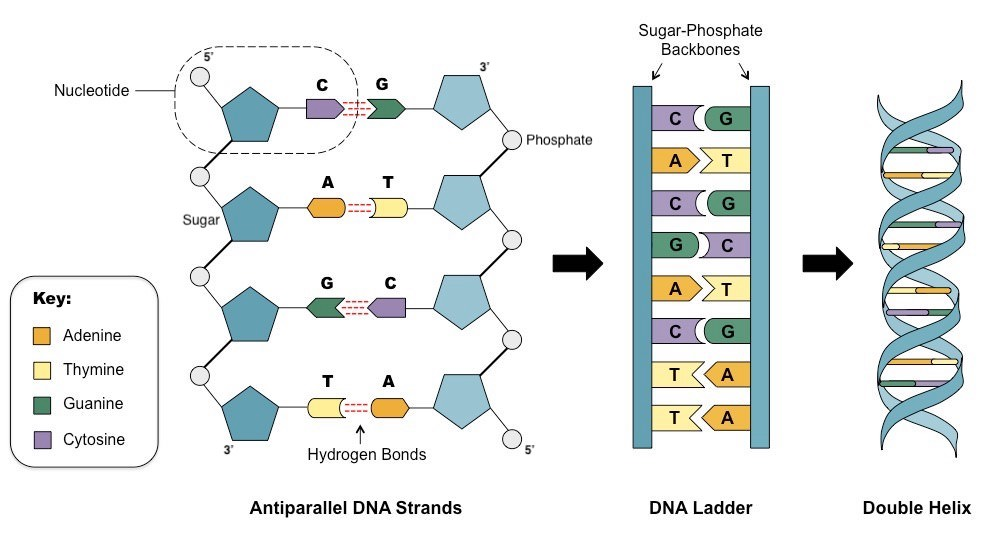
\includegraphics[width=0.8\textwidth]{dna-structure}
    \caption{DNA structure}
    \label{fig:dna-structure}
\end{figure}

Desoxyribonucleic acid (DNA) is a chemical molecule composed of two polynucleotide chains that coil around each other to form a double helix. DNA is the primary information carrier in living organisms and as such, it is the building block of all life. It holds the essential instructions for the development, maintenance and reproduction of all known organisms and many viruses. 

The two polynucleotides chains are composed of monomeric units called nucleotides, as described on Figure \ref{fig:dna-structure}.
Each nucleotide is built from one of the four nitrogen bases (adenine [A], cytosine [C], guanine [G] and thymine [T]), a sugar called deoxyribose and a phosphate group.
The nucleotides are linked to one another in a chain by a covalent bond between the sugar of one nucleotide and the phosphate group of the next, resulting in a alternating sugar-phosphate backbone.
The nucleotides of the two separate chains are joined together by an hydrogen bond between their nitrogen bases according to base pairing rules (A-T, G-C), creating the aformentioned double helix.
The nitrogen bases are divided into two groups, the pyrimidine bases (C and T) and the purine bases (A and G).

Both strands of DNA store the same information, in complementary pairs. The two strands of DNA run in opposite directions and are thus anti-parallel. The direction is determined by the 5' to 3' or 3' to 5' direction.

\subsection{Usage}

DNA is a powerfull tool for storing information for biological systems so it can also find its place in the synthetic DNA storage.
DNA storage can be used for applications that require for example:

\begin{itemize}
    \item \textbf{High information density}:
In 2017, scientists at Columbia University and the New York Genome Center published a method which allows perfect retrieval of information from a density of $215$ petabytes per gram of DNA \cite{bib:erlich_yaniv_2017_889697};
    \item \textbf{Data longevity}: Information stored in DNA can last for decades or centuries compared to conventional media which are replaced every 3-5 years \cite{bib:33649304};
    \item \textbf{Low energy consumption}: DNA does not use energy to store information, energy is only used to prevent the degradation of the DNA;
    \item \textbf{Ease of replication}: Thanks to the Polymerase Chain Reaction, DNA can be replicated easily \cite{bib:Mullis_1990}.
\end{itemize}

\subsection{End-to-end DNA storage}

\begin{figure}
    \centering
    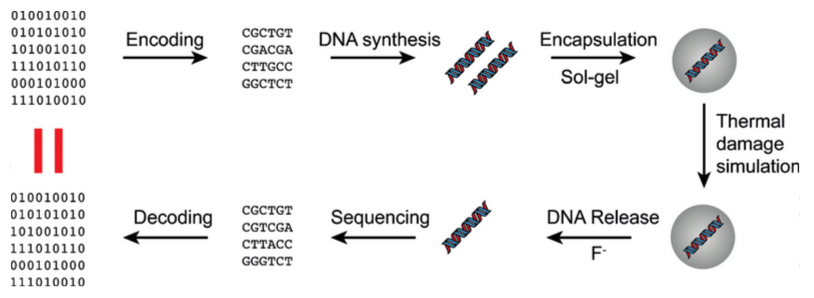
\includegraphics[width=0.6\textwidth]{dna-storage-pipeline}
    \caption{DNA storage pipeline}
    \label{fig:dna-storage-pipeline}
\end{figure}


The way to store binary information into DNA based medium storage and then retrieve it back is called end-to-end DNA storage. It has several steps as seen on Figure~\ref{fig:dna-storage-pipeline}.

\begin{itemize}
    \item \textbf{Encoding}: Transform any kind of information into a nucleotide stream (A, C, G or T);
    \item \textbf{Synthesis}: Synthesise the nucleotide stream into an actual DNA molecule;
    \item \textbf{Encapsulation}: Encapsulate the DNA molecule into a DNA medium for long term storage;
    \item \textbf{Thermal damage}: The DNA medium can be damaged by thermal damage, this can cause the DNA to break or be damaged during the storage process;
    \item \textbf{Release}: The DNA molecules can be released from the medium, it gives us the ability to retrieve the information back.
    \item \textbf{Sequencing}: The DNA molecules are sequenced on a computer, this allows us to digitally retrieve the information back as DNA sequences.
    \item \textbf{Decoding}: The DNA sequences are decoded back into the original information.
\end{itemize}

\subsection{Constraints}

Unfortunately, nucleic acids have biological constraints and can not be assembled in any order like it is the case for binary digits. The DNA strands have to be created in a way that the double helix binds well together and is not immediately desctructed. We must therefore respect the biological constraints to build strong strands that can last for a certain period of time. 

In this part, we are going to go through some of the constraints that we have to respect to build a DNA strand and be able to recover it during sequencing time. Unfortunately, the list of constraints is not exhaustive and in the real life, each arrangement of nucleic acids has an impact on the strength of a strand, therefore we can only simulate the longevity of a strand thanks to the actual litterature breakthroughs but not strictly respect all the biological constraints. 

All constraints could be reduced to limitations regarding GC content, long strands of a single nucleotide (so-called homopolymers), several repeated subsequences in a strand and motifs with biological relevance. In the next sections, we are going to divide the constraints into each step of the storage process, the explanation for each constraint comes directly from \cite{bib:10.1093/bioinformatics/btaa140}.

\subsubsection{Synthesis}

To synthesis synthetic DNA, \textit{in silico} designed constructs have to be split into smaller fragments [usually 200–3000 base pairs (bp)] \cite{bib:101038}. The fragments are then split into several oligonucleotides (so-called oligos) [usually 40-200 bp] that are individually synthetized. Once synthetized, all oligos are merged back together with either ligase or polymerase-based methods. One of the constraints on the GC content comes from the fact that depending on the synthetis method and the overall GC content of a fragment,  the GC content of each oligo has to be within a specific range. In oligos with high GC content, neighboring guanines tend to form an increased amount of hydrogen bonds, leading to inter/intra-strand folding \cite{bib:101371}.
To assemble oligos into larger fragments, the melting temperature (and thus the GC content) should only deviate slightly between oligos. To adhere to this restriction, the designed DNA fragments should be homogenous with respect to GC content. Homopolymers further increase the synthesis complexity, leading to fragments that are only synthesizable by using modified oligos and more sophisticated assembly methods, resulting in increased synthesis costs.

\subsubsection{PCR: Polymerase Chain Reaction}

The amplification of DNA using polymerase chain reaction (PCR) is indispensable for biological science. From DNA synthesis over cloning to DNA sequencing, PCR is used in a wide range of applications. 
One important factor of a successful PCR is the base composition of the amplification substrate. High melting temperatures due to high GC content of the DNA fragments hinder the separation of strands during the denaturation phase of the PCR. 
This reduces the yield of the PCR process, since the polymerase cannot efficiently synthesize the growing strand in the presence of previously existing hydrogen bonds. 
Stretches of repetitive DNA or high GC content can lead to the formation of secondary structures, hindering the elongation of the growing strand. 
Repetitive regions, as well as homopolymers, can also lead to polymerase slippage, a process in which polymerase briefly loses the connection to the template strand and reconnects at a different position with similar nucleotides content \cite{bib:102144} (a nice explanation can be seen \href{https://yewtu.be/watch?v=nRPNJ1T-ggg}{here}).

\subsubsection{Storage}

Further restrictions on the composition of the DNA construct are due to the cloning process: the GC content should be close to the GC percentage of the host genome and motifs used for the cloning process have to be avoided during the design of the DNA construct.

\subsubsection{Sequencing}

The base composition of a DNA fragment is also an important factor for the successful retrieval of genetic information using DNA sequencing technologies.
Illumina sequencing, Oxford Nanopore and PacBio sequencing technologies are biased toward DNA with an intermediate GC content, leading to reduced coverage of regions with strongly deviating GC content \cite{bib:101093}. 
Illumina and Nanopore sequencers also show an increased error rate in the presence of homopolymers \cite{bib:101093}.
Depending on the sequencing method used, the resulting data show increased substitution rates for specific DNA patterns: for PacBio data, common substitution patterns are CG $\rightarrow$ CA and CG $\rightarrow$ TG, Nanopore data contain an increased amount of TAG $\rightarrow$ TGG and TAC $\rightarrow$ TGC substitutions \cite{bib:1012688} and a common substitution pattern in Illumina data is GGG $\rightarrow$ GGT \cite{bib:101186}.

\subsection{MESA: Mosla Error Simulator}

In order to simulate without going through an expensive and long process that is DNA synthesis and sequencing, we are going to use a simulator that takes into account a large majority of biological constraints.
This simulator has been introduced \cite{bib:10.1093/bioinformatics/btaa140} in March 2020 and is a web application for the assessment of DNA fragments in terms of guanine-cytosine (GC) content, homopolymer occurrences and length, repeating subsequences and undesirable sequence motifs.
Furthermore, MESA contains a mutation simulator, using either the error probabilities of the assessment calculation, literature-based or user-defined error rates and error spectra. MESA is fully customizable using an easy-to-use web interface. All functionalities of MESA is also contained in a REST API, enabling the incorporation of MESA evaluations into custom workflows for high-throughput evaluation and error simulation of DNA.

As we have seen in the previous section, DNA has a lot of constraints during the synthesis, storage, PCR and sequencing step; With this simulator it is now possible to have a feedback of the strength of a particular DNA strand and thus help us to move towards the best DNA coding to ensure good information retrieval in the end.

